% ARPEGOS:  Automatized Roleplaying-game Profile Extensible Generator Ontology based System %
% Author : Alejandro Muñoz Del Álamo %
% Copyright 2019 %

% Section 2.2: Estado del Arte %

\section{Estado del Arte} \label{Estado_Arte}
Con el objetivo de simplificar el proceso de creación de personajes en los juegos de rol tradicionales, se han originado 
multitud de aplicaciones con diferentes funciones y finalidades. \medskip

Algunas de las aplicaciones son referencias completas de los juegos, que sirven como elementos de consulta accesibles, 
rápidos y precisos. Un ejemplo de ello es \textit{\textbf{5e Character}}, que es una referencia completa de personajes 
para \textit{Dragones y Mazmorras, 5ª Edición}.\bigskip
% https://play.google.com/store/apps/details?id=com.dungeon.dev.a5echaracter&hl=en_US

\begin{figure}[H]
    \centering
    \begin{minipage}{0.38\textwidth}
        \centering
        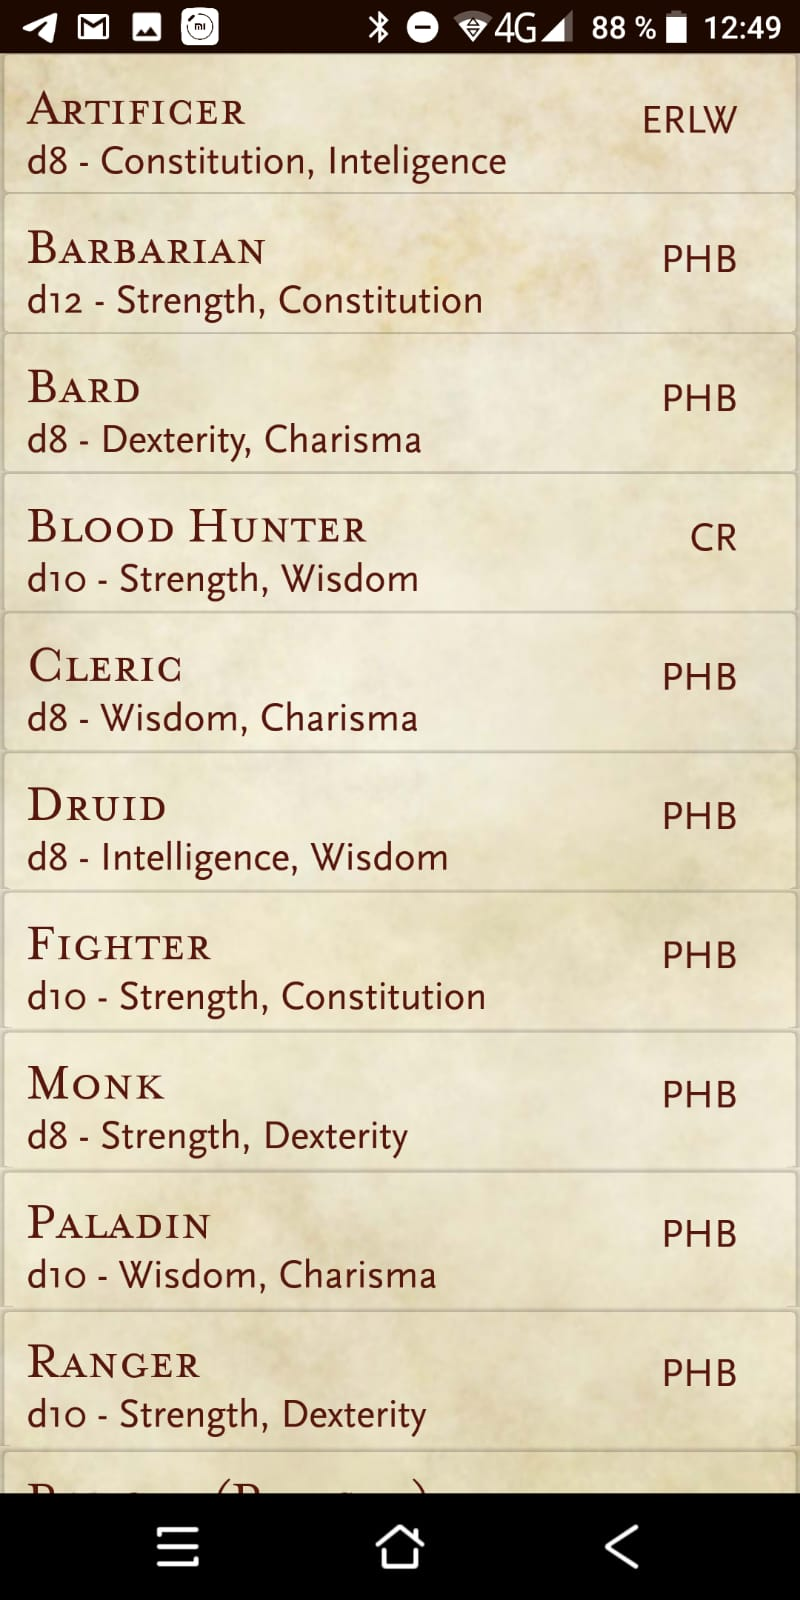
\includegraphics[width=0.5\textwidth]{Images/5e_Character_1.jpeg}
        \caption{\textit{\textbf{5e Character}}: Pantalla de selección 
        de clases}
        
    \end{minipage} \hspace{2cm}
    \begin{minipage}{0.38\textwidth}
        \centering
        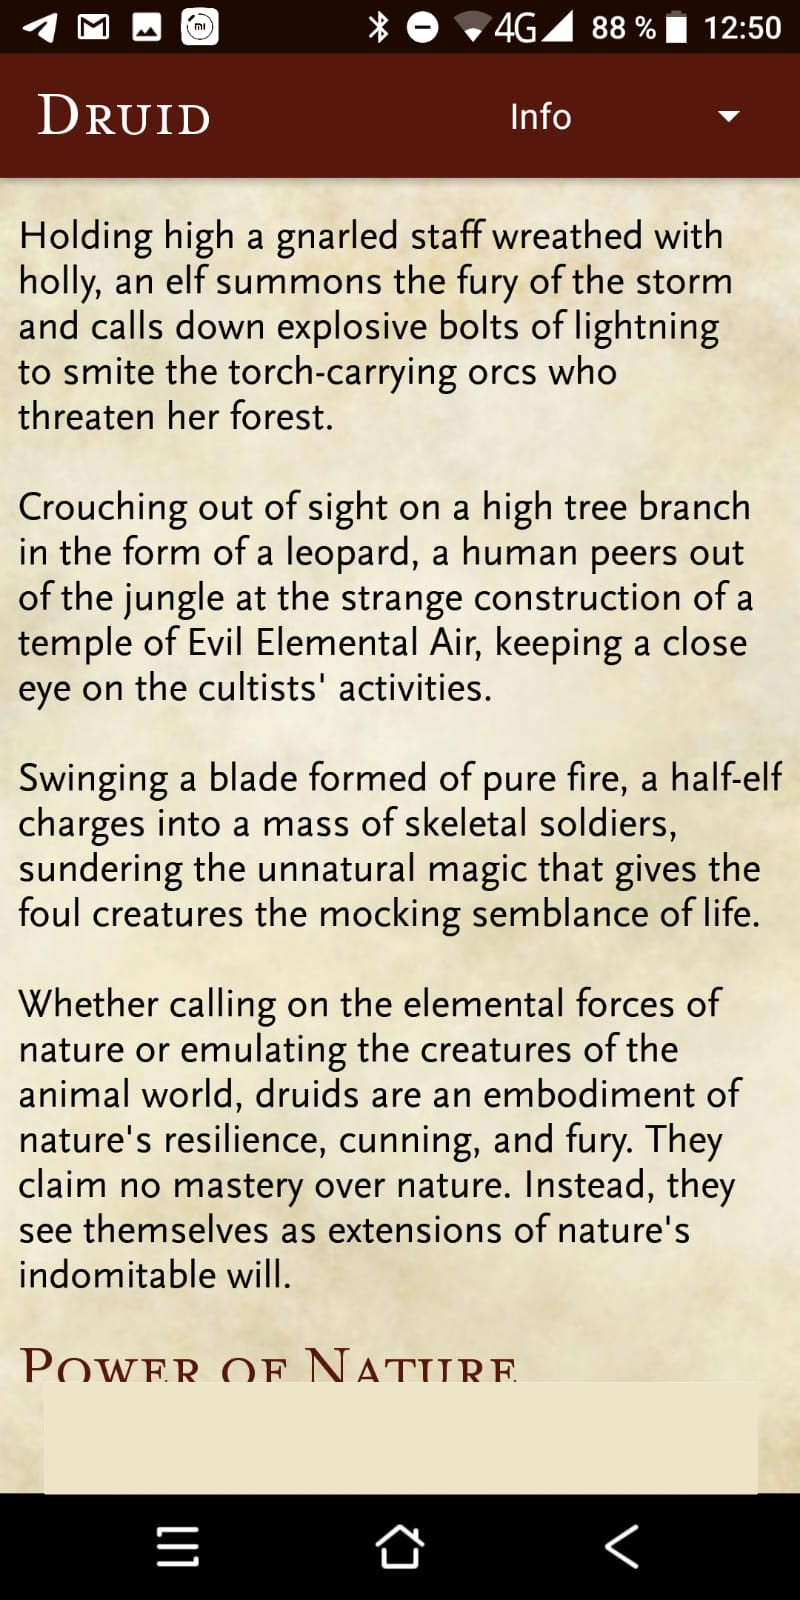
\includegraphics[width=0.5\textwidth]{Images/5e_Character_2.jpeg}
        \caption{\textit{\textbf{5e Character}}: Información 
        de la clase \textit{Druida}}
        
    \end{minipage}
\end{figure}

También podemos encontrar aplicaciones como \textit{\textbf{RPG Simple Dice}} 
que realizan simulaciones de lanzamiento de dados, en caso de que no 
dispongamos de dados físicos. \bigskip

\begin{figure}[H]
    \centering
    \begin{minipage}{0.35\textwidth}
        \centering
        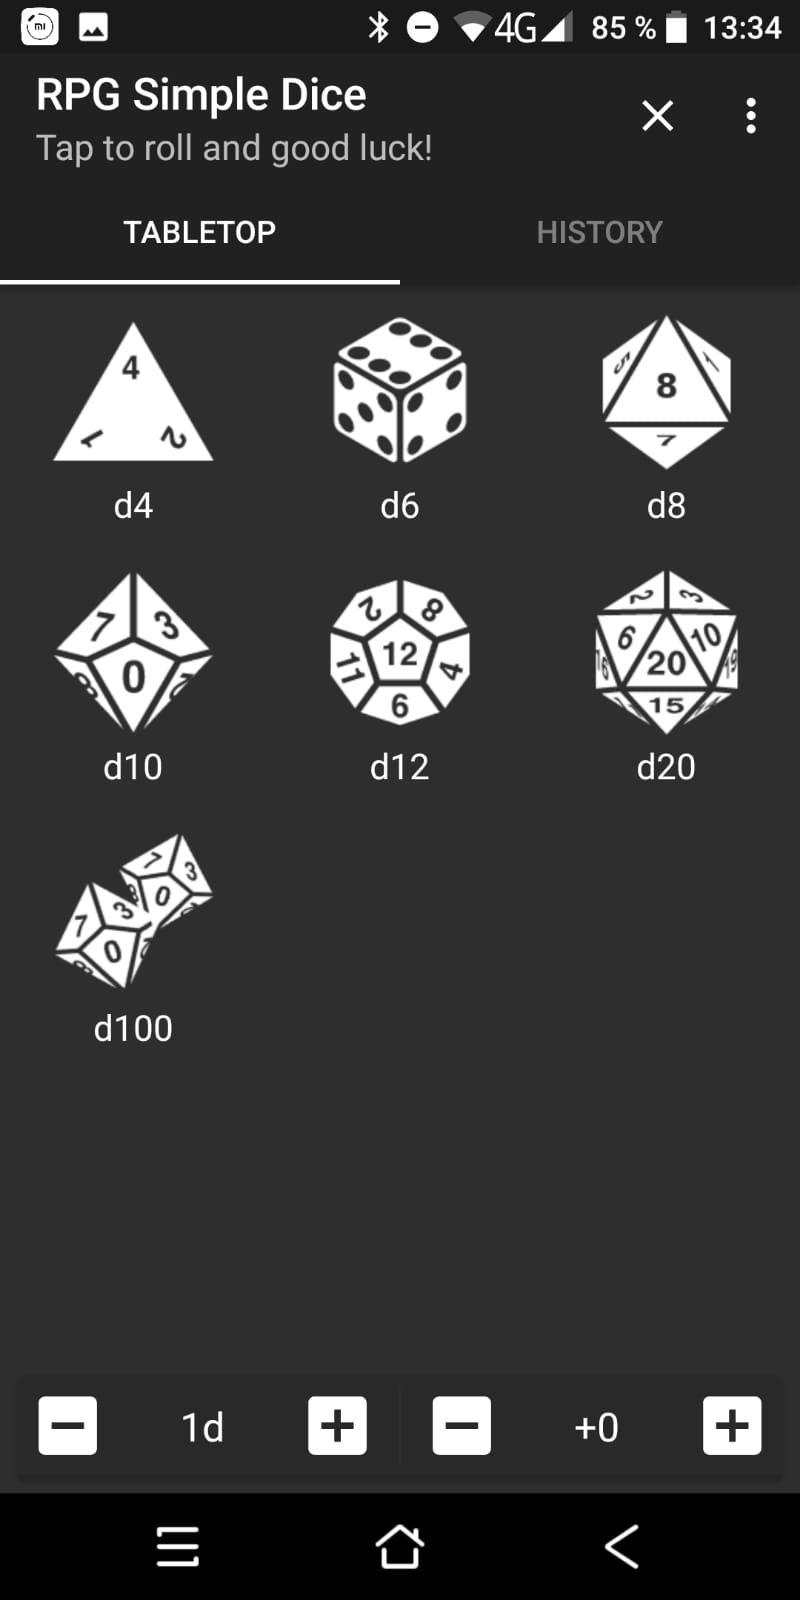
\includegraphics[width=0.5\textwidth]{Images/RPG_Simple_Dice_1.jpeg}
        \caption{\textit{\textbf{RPG Simple Dice}}: Pantalla de selección 
        de dados}
        
    \end{minipage} \hspace{2cm}
    \begin{minipage}{0.35\textwidth}
        \centering
        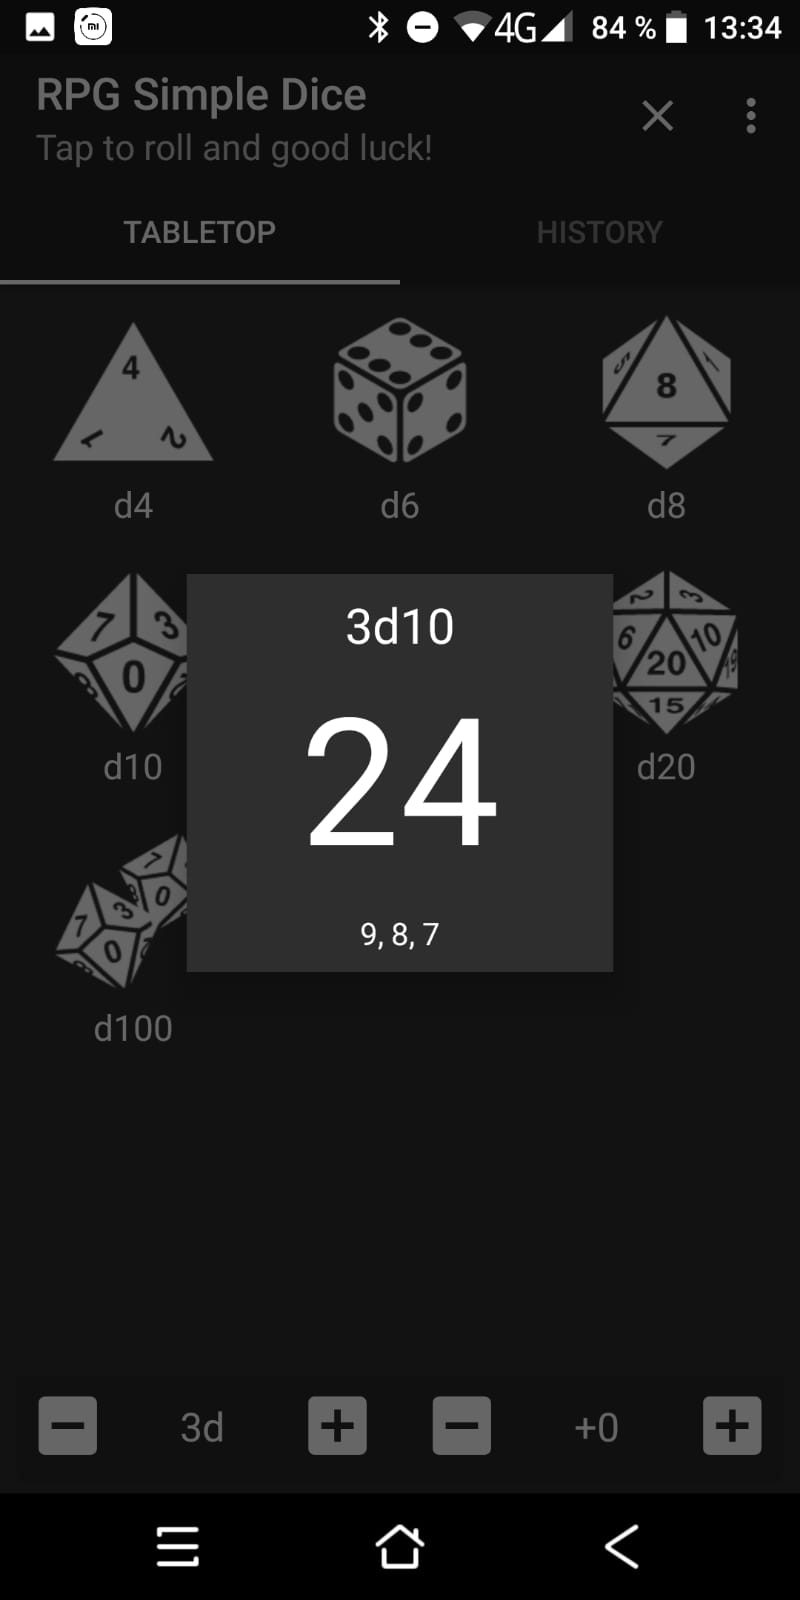
\includegraphics[width=0.5\textwidth]{Images/RPG_Simple_Dice_2.jpeg}
        \caption{\textit{\textbf{RPG Simple Dice}}: Ejemplo de lanzamiento de 
        dados}
        
    \end{minipage}
\end{figure}\bigskip

Otras en cambio, proporcionan algunas herramientas que simplifican algunos 
cálculos que resultan tediosos durante el transcurso de la partida, como 
es el caso de \textit{\textbf{BattleTrack}}. \bigskip

\begin{figure}[H]
    \centering
    \begin{minipage}{0.3\textwidth}
        \centering
        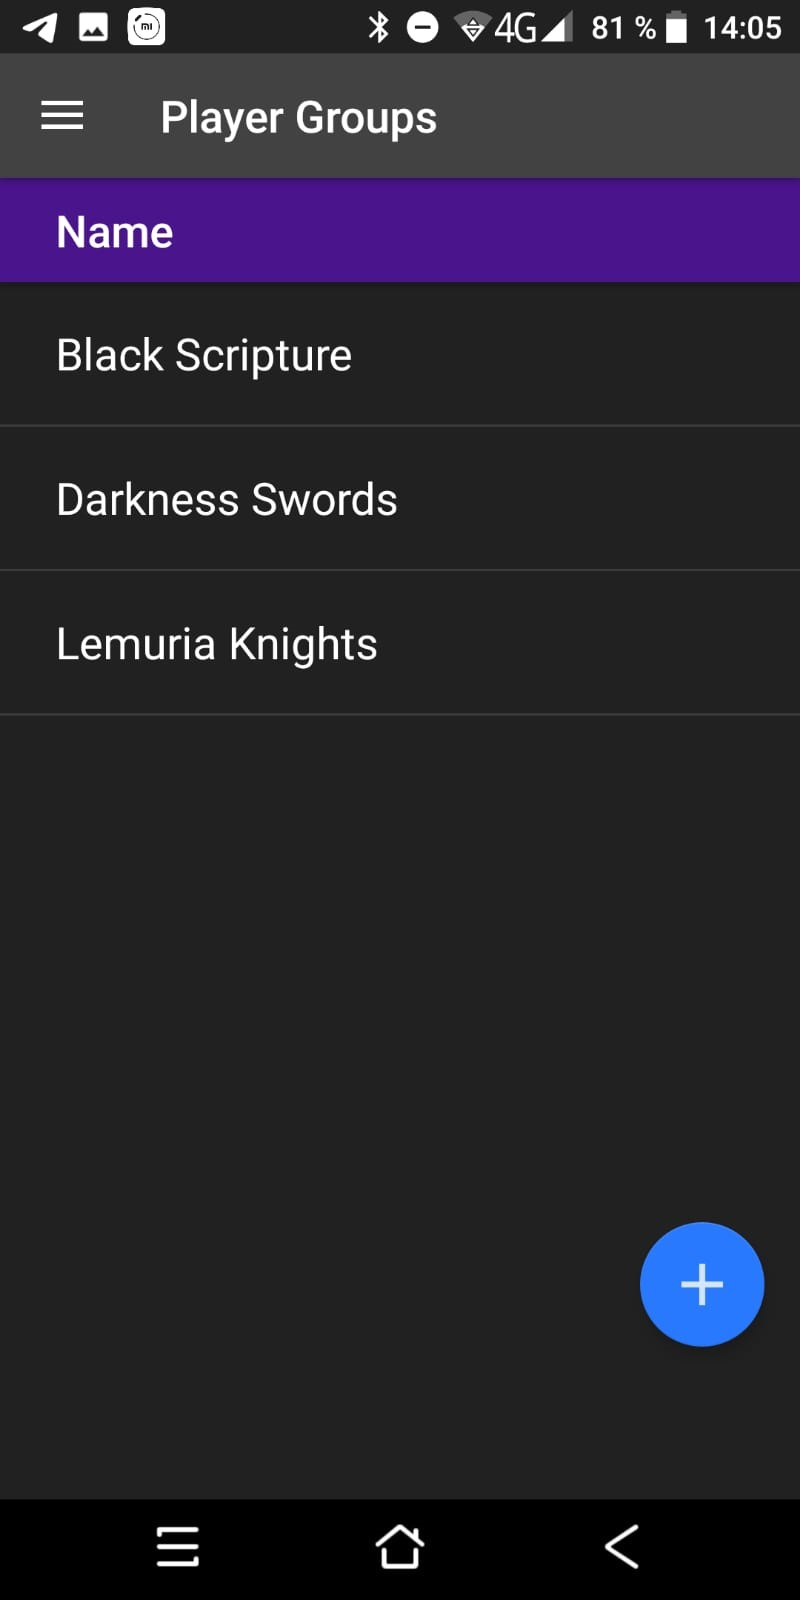
\includegraphics[width=0.7\textwidth]{Images/BattleTrack_1.jpeg}
        \caption{\textit{\textbf{BattleTrack}}: Pantalla de selección 
        de grupo}
        
    \end{minipage} \hspace{2cm}
    \begin{minipage}{0.3\textwidth}
        \centering
        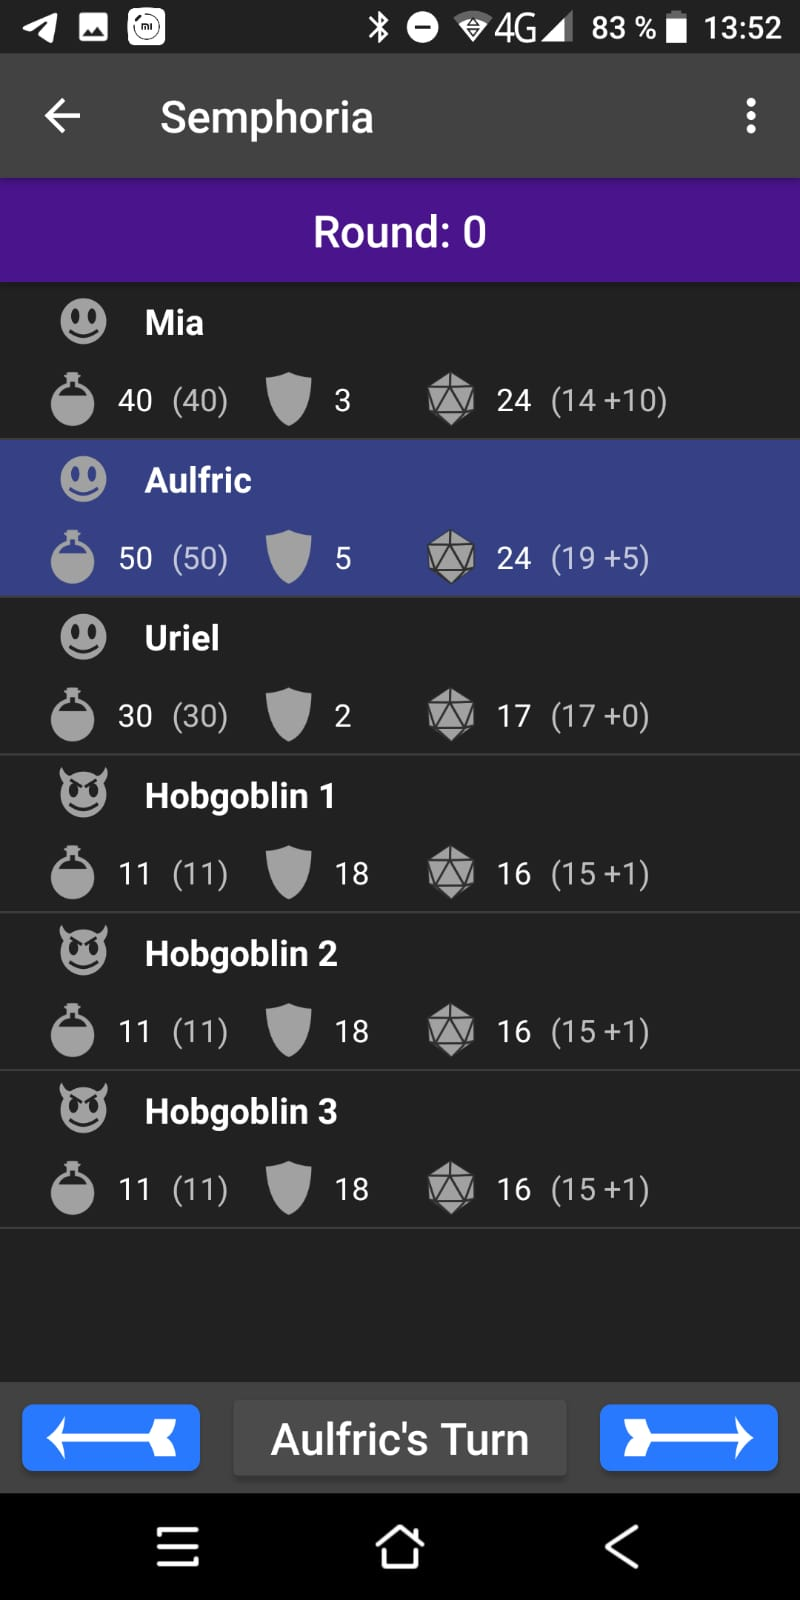
\includegraphics[width=0.7\textwidth]{Images/BattleTrack_2.jpeg}
        \caption{\textit{\textbf{BattleTrack}}: Ejemplo de combate}
        
    \end{minipage}
\end{figure}
\vspace{1cm}

Con el fin de ayudar en la ambientación, aplicaciones como 
\textit{\textbf{RPGSound}} aportan bibliotecas de sonido que se pueden 
utilizar durante la representación de la partida para sumirse en ella.\bigskip

\begin{figure}[H]
    \centering
    \begin{minipage}{0.3\textwidth}
        \centering
        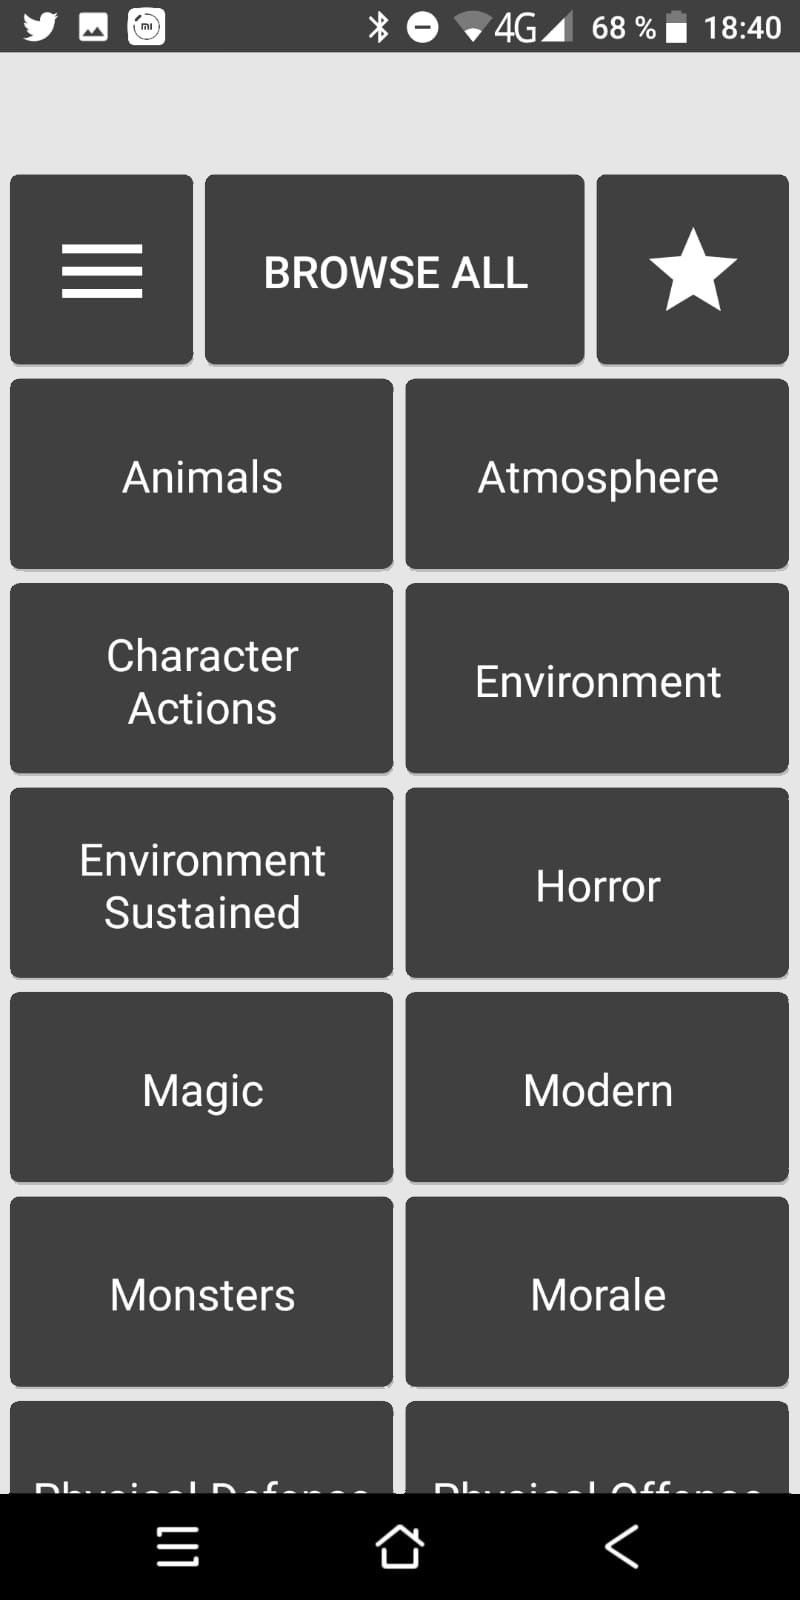
\includegraphics[width=0.7\textwidth]{Images/RPGSound_1.jpeg}
        \caption{\textit{\textbf{RPGSound}}: Menú principal}
        
    \end{minipage} \hspace{2cm}
    \begin{minipage}{0.3\textwidth}
        \centering
        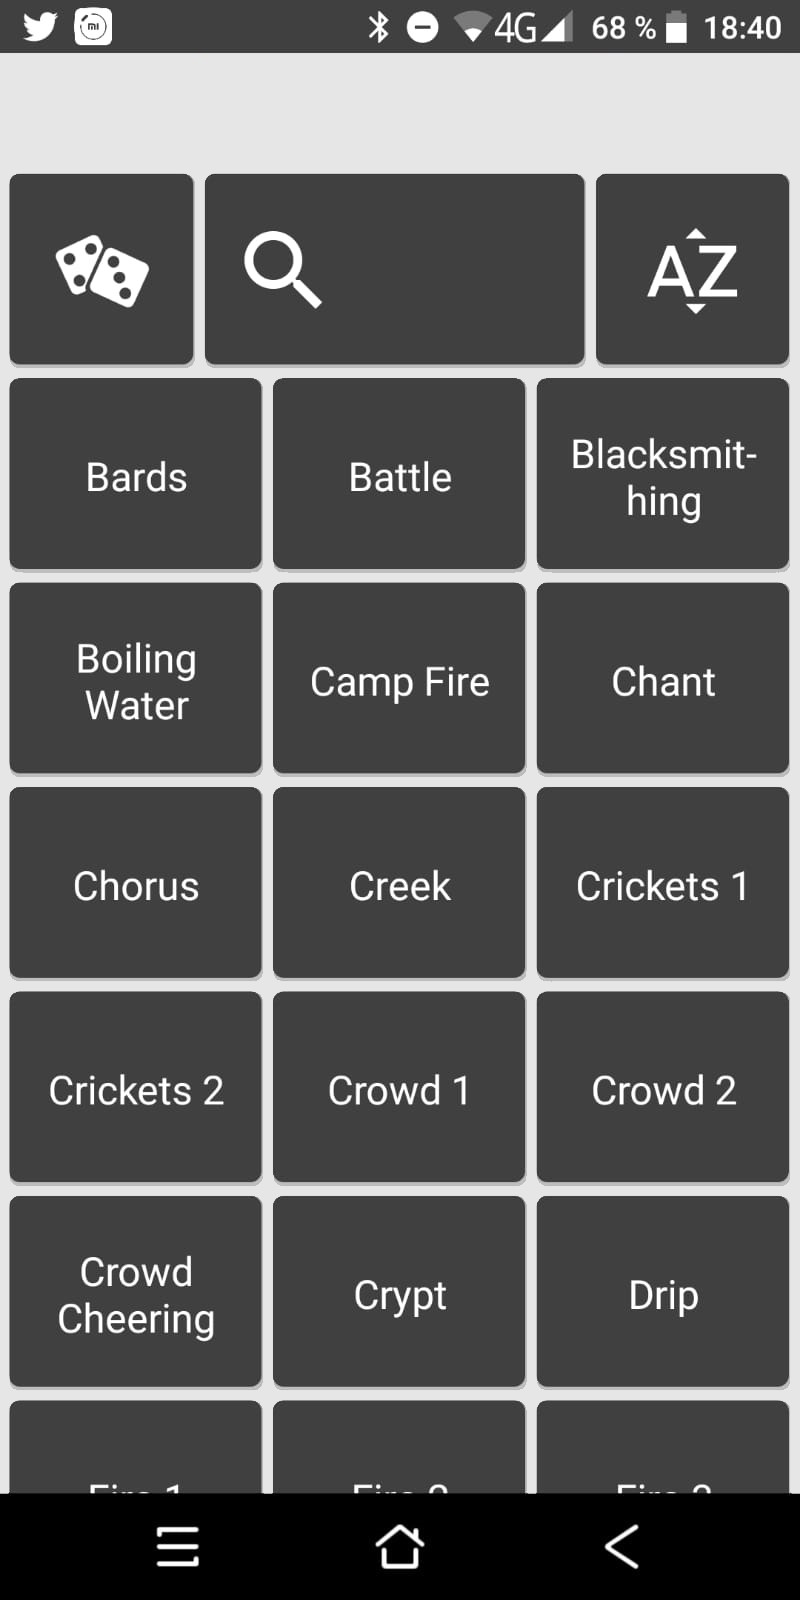
\includegraphics[width=0.7\textwidth]{Images/RPGSound_2.jpeg}
        \caption{\textit{\textbf{RPGSound}}: Menú de \textit{Ambiente 
        Sostenido}}
        
    \end{minipage}
\end{figure}\bigskip

Finalmente, quedan las aplicaciones conocidas como \textit{generadores de
personaje}, que permiten al usuario crear personajes para formar parte de 
una partida de rol, y acceder a esa información de forma rápida. Un buen 
ejemplo de esto es \textit{\textbf{RPG Character Sheet}}.\bigskip

\begin{figure}[H]
    \centering
    \begin{minipage}{0.3\textwidth}
        \centering
        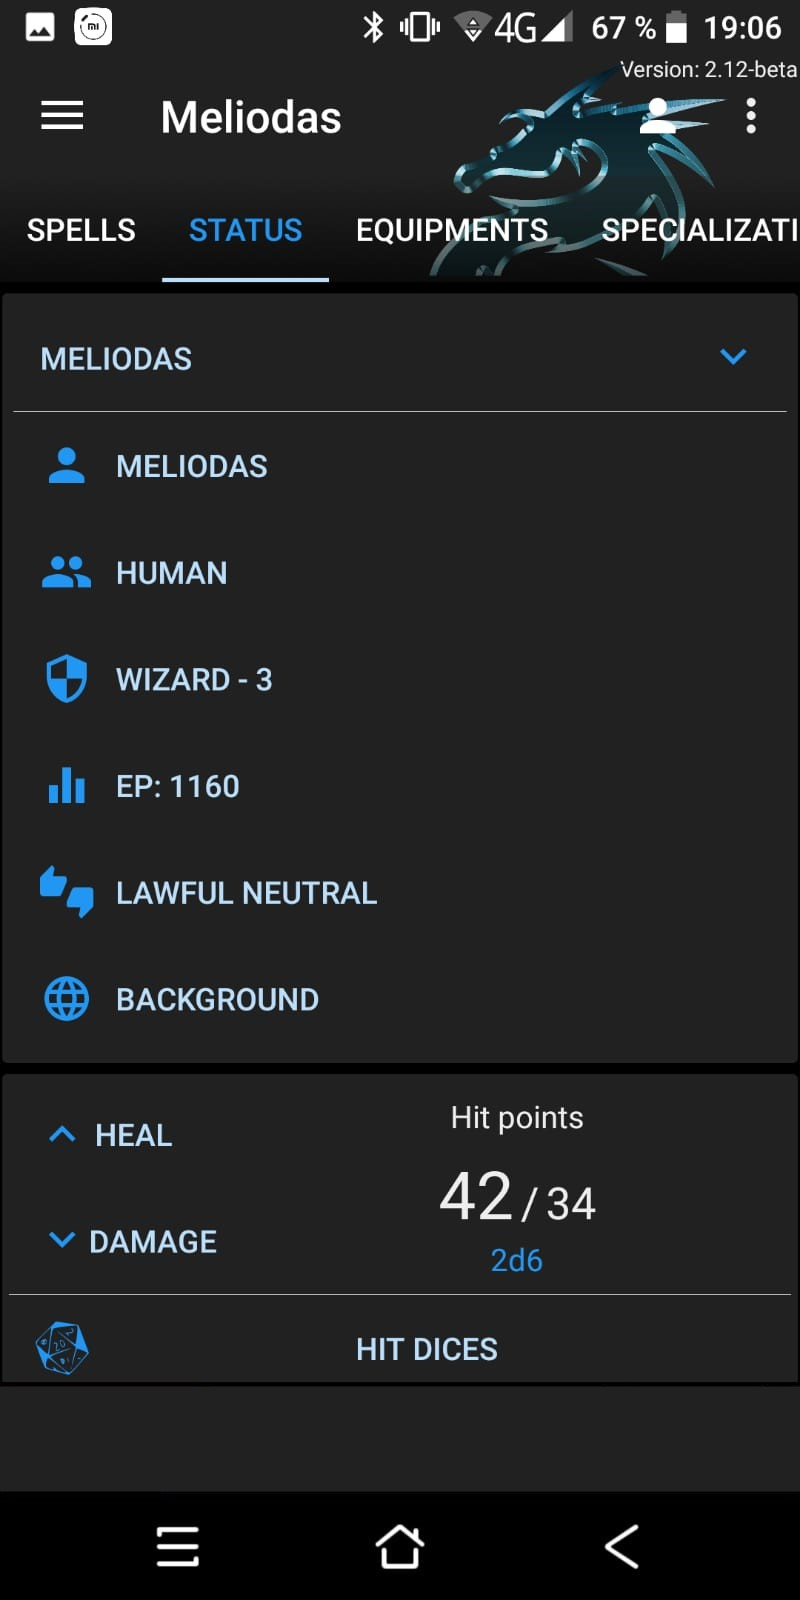
\includegraphics[width=0.7\textwidth]{Images/RPG_Character_Sheet_1.jpeg}
        \caption{\textit{\textbf{RPG Character Sheet}}: Pantalla de \textit{Estado}}
        
    \end{minipage} \hspace{2cm}
    \begin{minipage}{0.3\textwidth}
        \centering
        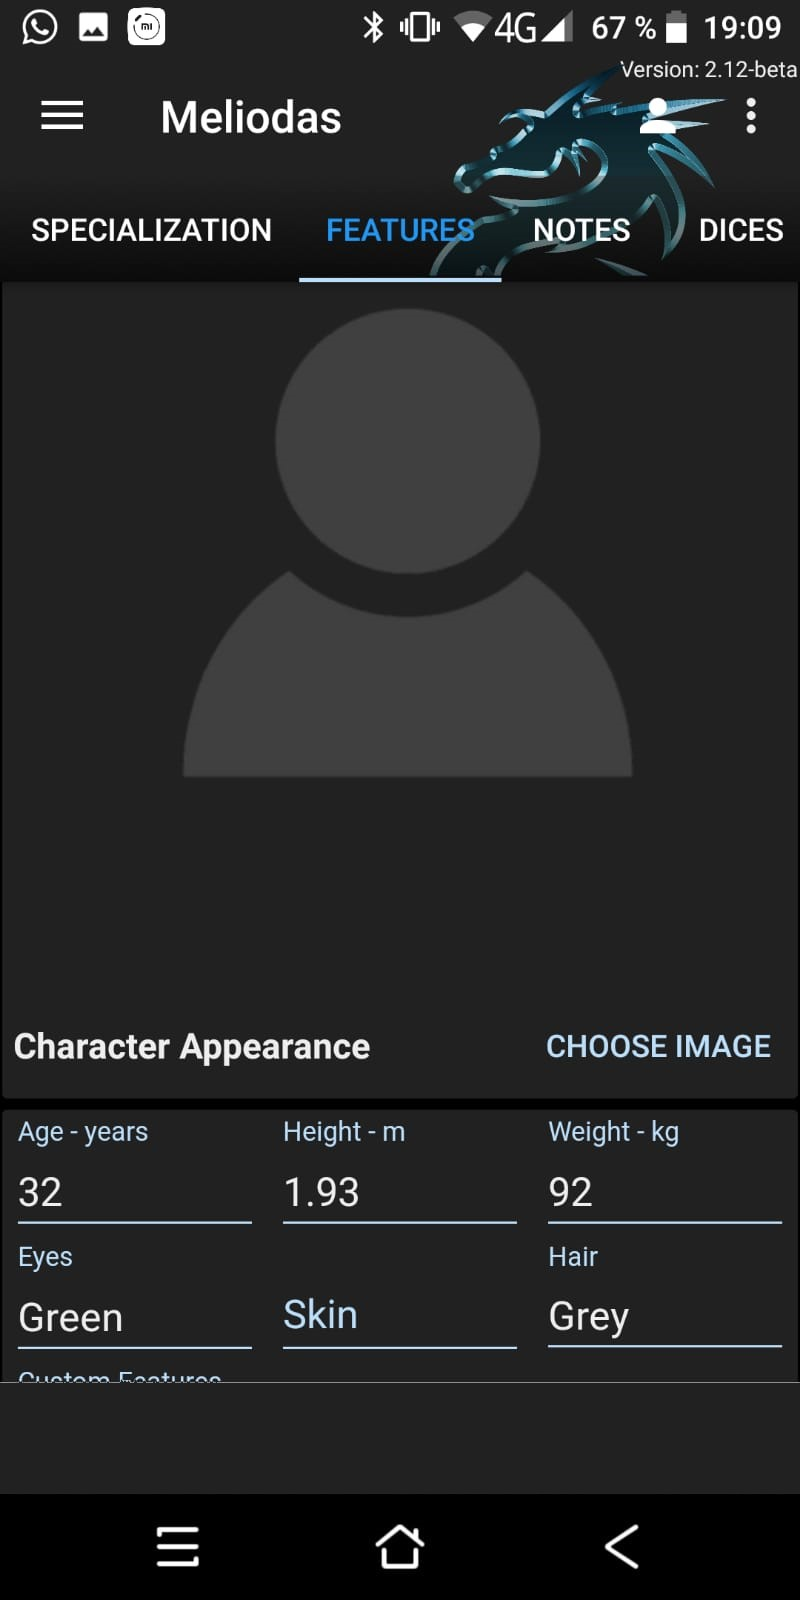
\includegraphics[width=0.7\textwidth]{Images/RPG_Character_Sheet_2.jpeg}
        \caption{\textit{\textbf{RPG Character Sheet}}: Pantalla de 
        \textit{Features}}
    \end{minipage}
\end{figure}